\section{Implementation}


\subsection{Structure}
\begin{center}
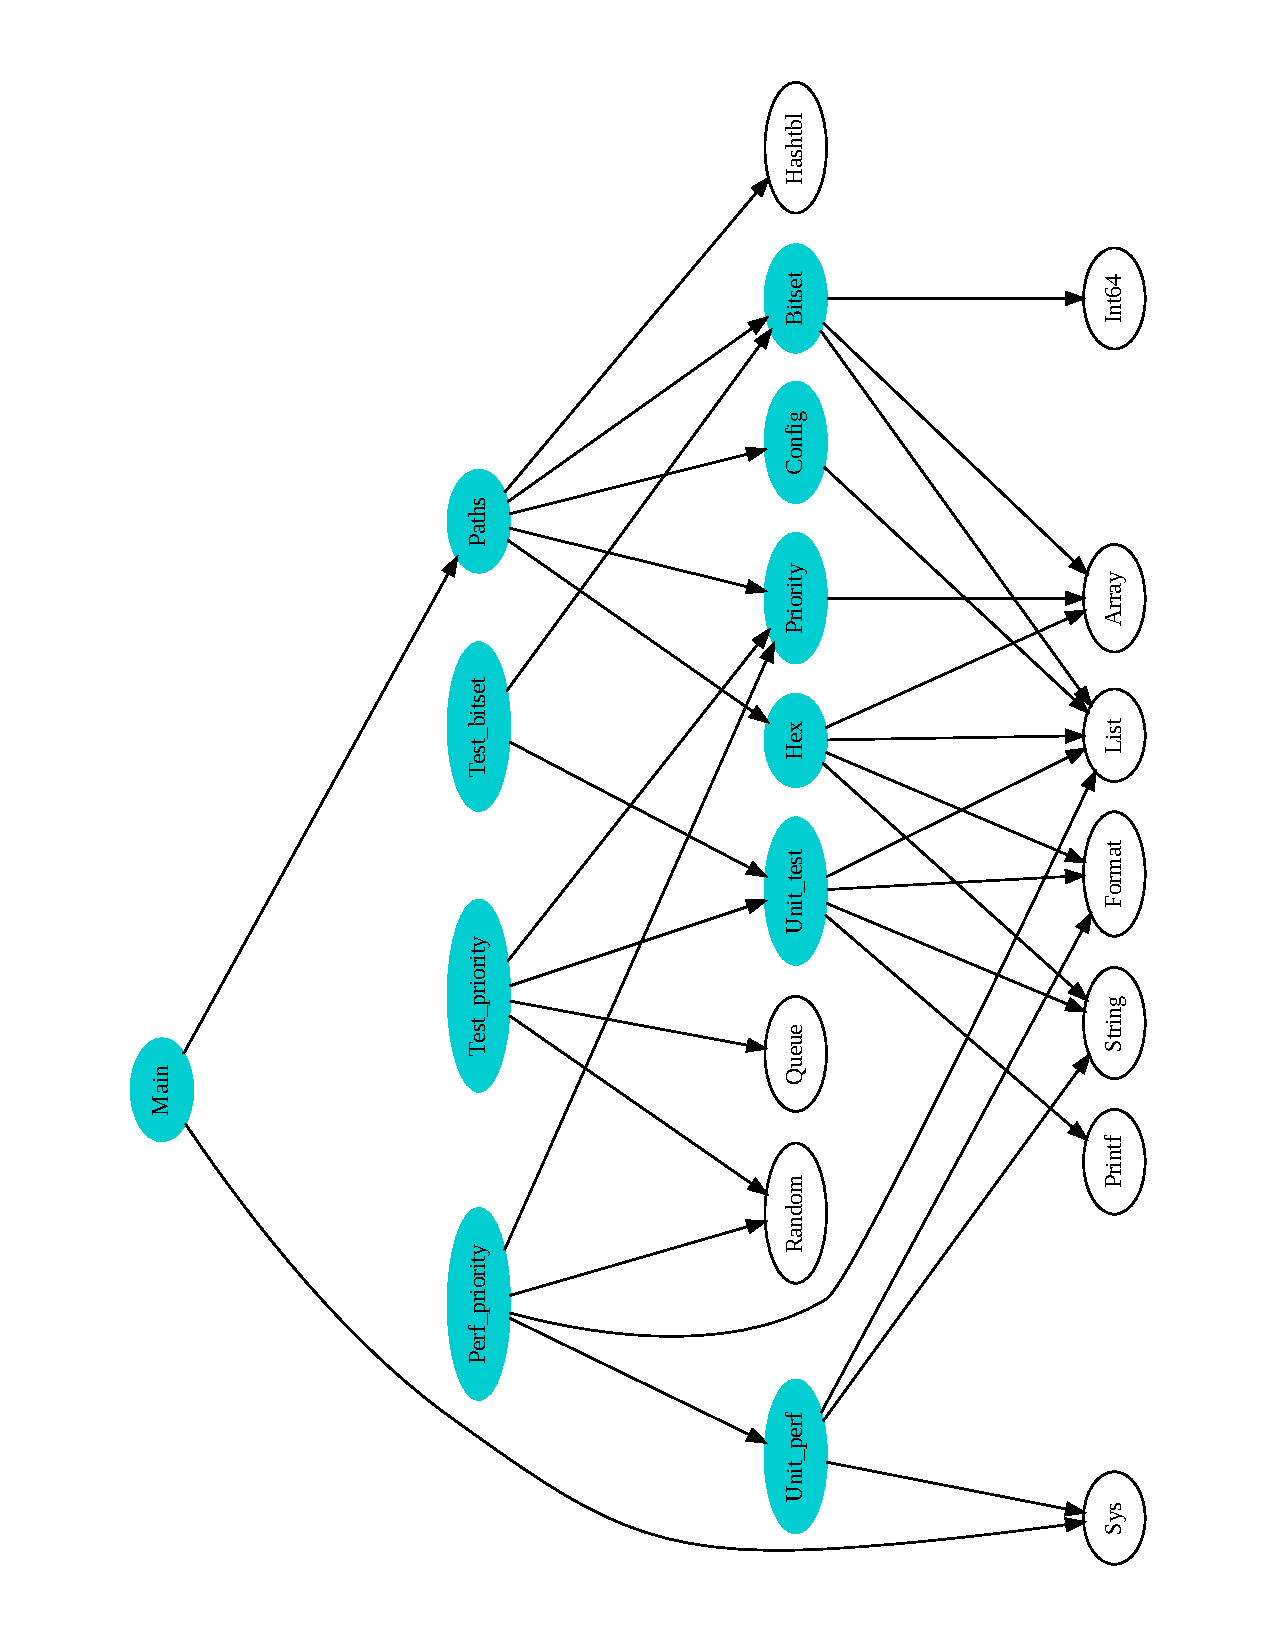
\includegraphics[width=8cm]{deps.pdf}
\end{center}


\subsection{\ttt{Hex}}

Directions were renamed to be more intuitive, and they were removed
from the public interface to be accessible only through \ttt{all\_directions}
and the utility functions \ttt{opposite} as well as \ttt{neighbors}.\\

\ttt{read\_grid} was made to be robust : it is able to read problems even
if they contain extra lines before \ttt{<problem>} or after \ttt{</problem},
and it is able to adapt itself depending on the parity of the line which
features indentation.


\subsection{\ttt{Bitset}}

\ttt{Bitset.t} uses \ttt{Int64.t} as recommended, and makes use of
bitwise operators for good performance.\\

Internally it uses mutable objects to avoid unnecessary copies but it exposes
an immutable public interface.\\

Several utility functions were added to implement standard operations that benefit
from not repeatedly converting from and to \ttt{int} and from avoiding creating
copies.\\
Those are \ttt{setminus}, \ttt{union}, \ttt{intersect} which are self-explanatory
both in name and in implementation as well as the more complex
\ttt{transitive\_closure} which takes a starting point and a \ttt{elt -> elt list}
neighbor function and calculates the connected component of \ttt{start}.\\
\ttt{compare} is useful to sort sets by increasing cardinal.


\subsection{\ttt{Priority}}

\ttt{'a node} was made with a mutable key so that \ttt{decrease\_key} does
not invalidate the reference handed out during \ttt{insert}.\\
\ttt{find} searches the location of the node in the queue to be used with
\ttt{member} and \ttt{remove}. \ttt{find} does not unnecessarily explore
the rest of the heap when it finds a key greater than the one being searched,
but no effort has been invested into any further improvement of performance,
since the two functions \ttt{remove} and \ttt{decrease\_key} are useless for
my implementation.\\

\ttt{sift} and \ttt{trinkle} perform rotations rather than two-element permutations
for some performance gain.\\


\subsection{\ttt{Paths}}

The finite type represents positions of \([0,\ttt{height}[ \times [0,\ttt{width}[\)
with the canonical bijection to \([0, \ttt{height}\times\ttt{width}[\).\\

\ttt{HMap} uses a static mutable \ttt{Hashtbl.t}, it is important to reset it before
an exploration to properly record the positions that have actually been explored.\\

Keys contain an upper bound on the final length of the path as well as its
current length.\\
Higher priority is given to configurations where the potential is greater, then
those whose computation is the most advanced.\\

A configuration \ttt{(remaining\_ice, current\_position)} is added to the list
of already explored configurations when it is time for its children to be added
to the priority queue.\\
This allows proving that \ttt{decrease\_key} is not required and that whenever a
position is marked as ``explored'' it is indeed unnecessary to consider it again.\\

Assume \ttt{(ice, pos)} is explored and that it is encountered again.\\
This means that two paths were found that lead to the same configuration.\\
Since the first one was considered first in the priority queue it must have
had higher potential at least up to the previous step. Since the configurations
are now the same, one of the following must be true :
(a) the two paths are not the same but have the same length,
(b) the first path has greater length.\\
If (a) is the case then the path cannot be strictly improved, and if (b) is the case
then the new path is worse than the previous one.\\
In both instances it is useless to calculate further.\\

An alternate way of interpreting the priority makes this fact obvious : sorting
keys by decreasing potential then by decreasing advancement makes the strategy to
be ``explore the current path as long as it doesn't waste any space, switch
to the next possible path as soon as going on with this path would require
sacrificing part of the positions''.\\
This fact explains the efficiency of the optimizations presented thereafter, of
which some seem counterintuitive.\\


